\chapter{Results and Discussion}
\label{chap:results}
    \section{OOV handling model}
        After training the model was done, some OOV words were fed
        into the model and 5 nearest in-vocabulary words were
        calculated for sanity check and shown on the table below. The
        input used were similar to the one used in testing
        \textsc{Mimick} on its original paper for Polyglot embedding
        for English and few examples from the brown corpus that turned
        out to be OOV, but only inputs that produced interesting
        results are shown. Both model CNN and \textsc{Mimick} results
        for nearest neighbor that were trained with Polyglot are shown
        in Table \ref{tab:nearest:cnn-polyglot} and Table
        \ref{tab:nearest:lstm-polyglot} respectively. The number of
        features for \textsc{Mimick} and CNN was 100.

        The first word was "hurtling", typographical error from the
        word hurting. For this word, both model seems to be able to
        locate that the nearest neighbor is another verb with suffix
        \textit{-ing}. Interestingly for CNN, it relates this word
        with action than might induce pain thus hurting a subject. The
        second word is "expectedly". Both model were able to predict
        that the nearest neighbor is another word with suffix
        \textit{-ly}. The third input word is "Actively". For this
        input, \textsc{Mimick} predicted that this word is a name
        which the first word is capitalize, thus the nearest neighbor
        is name. On the other hand, CNN predicted that this is some
        word with suffix \textit{-ly} and capital letter is used at
        the beginning. The next word is "corduroy", which is a pattern
        in textile. CNN model were able to predict that one of the
        nearest neighbor is "garment". The next input is
        "question-and-answer". This input constructed from 3 words
        connected with dash (-) symbol. CNN model predicted that the
        nearest neighbor were activities that the subjects do, for
        instance "hostess" and "recruiter". The last input is a number
        "1657". \textsc{Mimick} predicted that the nearest neighbor is
        mathematical function in latex for example "\textbackslash
        exp", while CNN predicted the nearest neighbor to be an
        abbreviation.

        From those results, both models were able to predict the
        nearest neighbor that might be related to each other for some
        cases, but this results are highly dependent on the pre-trained
        embedding that was used to train the OOV handling model. If both model
        were trained using Word2vec, then for input word "hurtling"
        and "corssing" produced nearest neighbor "turning", "putting",
        "squeezing", "pushing", "talking", and "pulling" in different
        order sorted from the closest to the furthest.
        
        % The first test word were an abbreviation "MCT" with length of
        % three characters and all-capitalize. Both model were able to
        % predict that the nearest neighbors are also another
        % abbreviation. For name as input, "McNeally" and "Vercelloti",
        % both model were able to predict the nearest neighbor to be
        % name as well, as shown on Table \ref{tab:nearest:cnn-word2vec}
        % and Table \ref{tab:nearest:lstm-word2vec}. For "McNeally" the
        % nearest neighbor were English name for male for both models.
        % Interestingly for "Vercellotti", \textsc{Mimick} predicted
        % that the nearest neighbor was former American baseball player,
        % while CNN predicted that the nearest neighbor was Ukrainian
        % politician. For an adjective input "Secretive", both model
        % were predicted that the nearest neighbors are group of verbs,
        % nouns, adjectives, and adverbs. Both models were also able to
        % handle typography error like "corssing" and "developiong",
        % only that CNN model nearest word were "developing" while
        % \textsc{Mimick} were a verb that has suffix \textit{-ing}. The
        % nearest neighbors for corssing were also verb with suffix
        % \textit{-ing}. Interestingly, for both model, nearest neighbor
        % for flatfish has no correlation at all.

        % Similar nearest neighbors were also produced by the model when
        % trained with polyglot \citep{polyglot2013alrfou} only with
        % different set of words for each input.

        \begin{table}[H]
          \begin{center}
            \caption{Nearest Neighbors Mimick (Polyglot)}
            ~\\
            \footnotesize
            \label{tab:nearest:lstm-polyglot}
            \begin{tabular}{l|l}
              \textbf{Word} & \textbf{Nearest Neighbors}\\
              \hline
              hurtling & inflating compromising concealing grasping channeling\\
              expectedly & materially substantively sensibly energetically ethically\\
              Actively & Harrold Wasson Wheatcroft Dever Covey\\
              corduroy & heartbeat kink delicacy diaper damper\\
              question-and-answer & barometer bottleneck ventilator slowdown spurt\\
              1657 & \textbackslash exp \textbackslash frac\{n \textbackslash frac\{\# sqrt x\^{}\{\\
            \end{tabular}
          \end{center}
        \end{table}

        \begin{table}[H]
          \begin{center}
            \caption{Nearest Neighbors CNN (Polyglot)}
            ~\\
            \footnotesize
            \label{tab:nearest:cnn-polyglot}
            \begin{tabular}{l|l}
              \textbf{Word} & \textbf{Nearest Neighbors}\\
              \hline
              hurtling & pulling whipping catching shaking burning\\
              expectedly & frequently legitimately painfully inappropriately purposefully\\
              Actively & Easily Potentially Entirely Merely Displaying\\
              corduroy & basket garment wedge medium nutrient\\
              question-and-answer & hostess dentist recruiter carer pastime\\
              1657 & GER BO INT SEP AGP\\
            \end{tabular}
          \end{center}
        \end{table}

        % \begin{table}[H]
        %   \begin{center}
        %     \caption{Nearest Neighbors Mimick (word2vec)}
        %     ~\\
        %     \footnotesize
        %     \label{tab:nearest:lstm-word2vec}
        %     \begin{tabular}{l|l}
        %       \textbf{Word} & \textbf{Nearest Neighbors}\\
        %       \hline
        %       MCT & AWS NIC BTC ATS AAR\\
        %       McNeally & Wagstaff Lanning O'Dell Kellman Wolk\\
        %       Vercellotti & Antonelli Cardinale Veron Villani Sabatini\\
        %       Secretive & Entrepreneurial Predictive Screening Routine Themed\\
        %       corssing & compromising balancing inflating pulling reversing\\
        %       flatfish & slimy fluffy supple flaky greasy\\
        %       compartmentalize & formalize scrutinize validate redefine formulate\\
        %       pesky & nutty sensuous dreamy pungent euphoric\\
        %       lawnmower & lifeguard laborer tradesman bathhouse boarder\\
        %       developiong & compromising channeling sacrificing cementing alienating\\
        %       hurtling & pounding pulling catching compromising whipping\\
        %       expectedly & painfully strangely admirably energetically legitimately\\
        %       prople & figure circle mask plot pattern\\
        %       nrews & counters messes tips dials timings\\
        %       newss & promise knack friendliness hype bounce\\
        %       googel & wand contraption handkerchief talisman noose\\
        %     \end{tabular}
        %   \end{center}
        % \end{table}
        
        % \begin{table}[H]
        %   \begin{center}
        %     \caption{Nearest Neighbors Mimick (Polyglot)}
        %     ~\\
        %     \footnotesize
        %     \label{tab:nearest:lstm-word2vec}
        %     % \setlength\extrarowheight{2pt}
        %     \begin{tabularx}{1.1\textwidth}{|c|L|c|L|}
        %       \hline
        %       \textbf{OOV} & \textbf{Nearest Neighbors} & \textbf{OOV} & \textbf{Nearest Neighbors}\\
        %       \hline
        %       MCT & AWS NIC BTC ATS AAR & McNeally & Wagstaff Lanning O'Dell Kellman Wolk\\ \hline
        %       Vercellotti & Antonelli Cardinale Veron Villani Sabatini & Secretive & Entrepreneurial Predictive Screening Routine Themed\\  \hline
        %       corssing & compromising balancing inflating pulling reversing & flatfish & slimy fluffy supple flaky greasy\\  \hline
        %       compartmentalize & formalize scrutinize validate redefine formulate & pesky & nutty sensuous dreamy pungent euphoric\\  \hline
        %       lawnmower & lifeguard laborer tradesman bathhouse boarder & developiong & compromising channeling sacrificing cementing alienating\\ \hline
        %       hurtling & pounding pulling catching compromising whipping & expectedly & painfully strangely admirably energetically legitimately\\ \hline
        %       prople & figure circle mask plot pattern & nrews & counters messes tips dials timings\\ \hline
        %       newss & promise knack friendliness hype bounce & googel & wand contraption handkerchief talisman noose\\ \hline
        %     \end{tabularx}
        %   \end{center}
        % \end{table}
        
        % \begin{table}[H]
        %   \begin{center}
        %     \caption{Nearest Neighbors CNN (word2vec)}
        %     ~\\
        %     \small
        %     \label{tab:nearest:cnn-word2vec}
        %     \begin{tabular}{c|l}
        %       \textbf{Word} & \textbf{Nearest Neighbors}\\
        %       \hline
        %       MCT & DPP PCT PMC TSMC RTA\\
        %       McNeally & Murphy McCullough McIntyre Gallagher Delaney\\
        %       Vercellotti & Yanukovych Tymoshenko Yushchenko Saakashvili Ancelotti\\
        %       Secretive & Important Acquisition Process Benefits Transactions\\
        %       corssing & putting turning squeezing pulling sneaking\\
        %       flatfish & Wasps Premiership footballing Saracens flavorful\\
        %       compartmentalize & efficiencies retrofit development commercialize integrate\\
        %       pesky & weird cranky goofy scary joked\\
        %       lawnmower & driveway sidewalk porch mother creek\\
        %       developiong & developing development develop reshaping investment\\
        %       hurtling & knocking chasing tearing ripping slamming\\
        %       expectedly & predictably certainly unbelievably amazingly quite\\
        %     \end{tabular}
        %   \end{center}
        % \end{table}

        
        
        % \begin{table}[H]
        %   \begin{center}
        %     \caption{Nearest Neighbors Mimick (polyglot)}
        %     ~\\
        %     \small
        %     \label{tab:nearest:lstm-polyglot}
        %     \begin{tabular}{c|l}
        %       \textbf{Word} & \textbf{Nearest Neighbors}\\
        %       \hline
        %       MCT & \multicolumn{1}{p{0.7\textwidth}}{NAL MIB AWS SIA SMP}\\
        %       McNeally & \multicolumn{1}{p{0.7\textwidth}}{McCready Hiatt Tolan McAdams Coxon}\\
        %       Vercellotti & \multicolumn{1}{p{0.7\textwidth}}{Aurich Cavour Gubbio Barcelos Camoes}\\
        %       Secretive & \multicolumn{1}{p{0.7\textwidth}}{Rhetorical Predictive Contextual Affective Perceptual}\\
        %       corssing & \multicolumn{1}{p{0.7\textwidth}}{inflating straining concealing compromising channeling}\\
        %       flatfish & \multicolumn{1}{p{0.7\textwidth}}{whirlpool cocoon diaper crevice gutter}\\
        %       compartmentalize & \multicolumn{1}{p{0.7\textwidth}}{reproducible quantifiable repeatable synergistic biologic}\\
        %       pesky & \multicolumn{1}{p{0.7\textwidth}}{waxy lozenge phosphor thermoplastic flake}\\
        %       lawnmower & \multicolumn{1}{p{0.7\textwidth}}{dishwasher caddy welder motorist rowboat}\\
        %       developiong & \multicolumn{1}{p{0.7\textwidth}}{compromising inflating loosening halting venting}\\
        %       hurtling & \multicolumn{1}{p{0.7\textwidth}}{splashing blasting shredding combing pounding}\\
        %       expectedly & \multicolumn{1}{p{0.7\textwidth}}{realistically energetically conspicuously materially imperfectly}\\
        %     \end{tabular}
        %   \end{center}
        % \end{table}

        % \begin{table}[H]
        %   \begin{center}
        %     \caption{Nearest Neighbors CNN (polyglot)}
        %     ~\\
        %     \small
        %     \label{tab:nearest:cnn-polyglot}
        %     \begin{tabular}{c|l}
        %       \textbf{Word} & \textbf{Nearest Neighbors}\\
        %       \hline
        %       MCT & \multicolumn{1}{p{0.7\textwidth}}{NDS TEN GTC CPO UNI}\\
        %       McNeally & \multicolumn{1}{p{0.7\textwidth}}{briefly quietly Akerman enthusiastically Coons}\\
        %       Vercellotti & \multicolumn{1}{p{0.7\textwidth}}{Hassel Lemaire Sarno Perrot Necker}\\
        %       Secretive & \multicolumn{1}{p{0.7\textwidth}}{Rhetorical Subjective Legitimate Contextual Constructive}\\
        %       corssing & \multicolumn{1}{p{0.7\textwidth}}{confining straining inflating impacting shrinking}\\
        %       flatfish & \multicolumn{1}{p{0.7\textwidth}}{narcotic transient hangover lameness stench}\\
        %       compartmentalize & \multicolumn{1}{p{0.7\textwidth}}{commercialisation numeracy alertness institutionalization practicality}\\
        %       pesky & \multicolumn{1}{p{0.7\textwidth}}{eyeballs jerky wrinkles fuss bruise}\\
        %       lawnmower & \multicolumn{1}{p{0.7\textwidth}}{lavatory washroom toilet restroom mattress}\\
        %       developiong & \multicolumn{1}{p{0.7\textwidth}}{distancing compromising orienting manoeuvring harmonizing}\\
        %       hurtling & \multicolumn{1}{p{0.7\textwidth}}{compromising confining inflating lightening channeling}\\
        %       expectedly & \multicolumn{1}{p{0.7\textwidth}}{substantively realistically sensibly procedurally irrevocably}\\
        %     \end{tabular}
        %   \end{center}
        % \end{table}

    \section{POS-tagging results}
      Before using the OOV handling model, random embedding for OOV
      entries were used to lay the baseline of the OOV handling method
      for POS-tagging. The OOV entries were added into the vocabulary
      list and their embedding were randomly initialized. This
      collection of embedding then trained in conjunction with the
      POS-tagger model. The results are shown in figure
      \ref{fig:postag_random_results}.
      \begin{figure}[H]
        \centering
        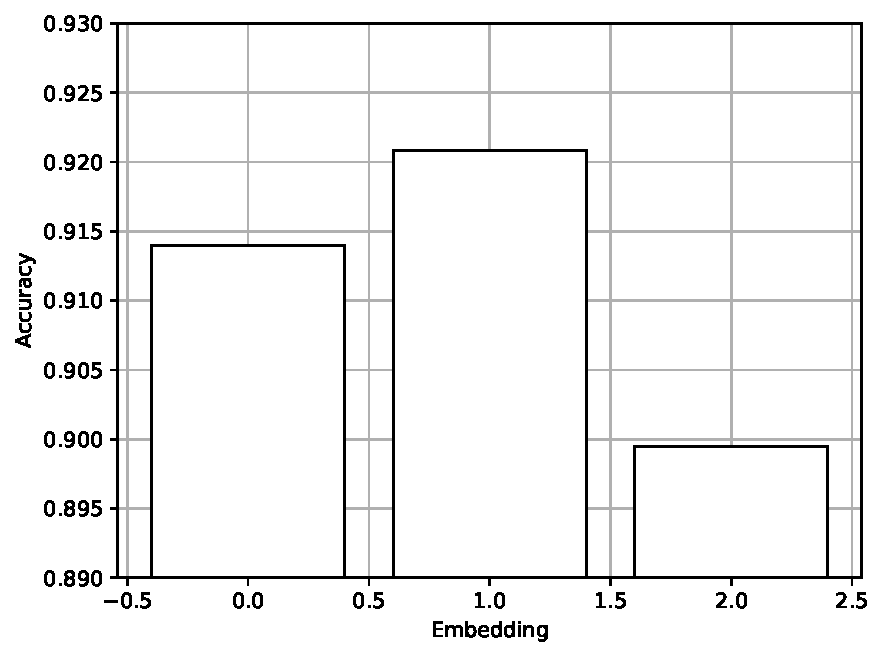
\includegraphics[width=0.8\linewidth]{images/random_graph.pdf}
        \caption{POS-tagging results with random OOV embedding}
        \label{fig:postag_random_results}
      \end{figure}

      In order to test the best number of features parameter for each
      OOV handling model, the model and the embedding were set to be
      in evaluation mode or frozen, meaning that the parameters will
      not change when training the POS-tagger model. The OOV embedding
      from both model on top of the pre-trained embedding were used as
      input for POS-tagging task. Firstly, the embedding for OOV
      entries were predicted through the OOV handling model and added to the
      pre-trained word embedding. Then the collection of the
      pre-trained embedding and the predicted OOV embedding weights
      were fixed so it would not be changed in the training process. The
      results of different number of features on different pre-trained
      embeddings are shown in figure
      \ref{fig:postag_word2vec_freeze_results}, figure
      \ref{fig:postag_polyglot_freeze_results}, and figure
      \ref{fig:postag_dict2vec_freeze_results}. With this settings,
      only CNN with 20 number of features can outperforms the
      \textsc{Mimick} model in Word2vec word embedding while
      \textsc{Mimick} performs better in the other word embedding
      across different number of features used. Interestingly, this
      setting for bot models perform worse than randomly initialized
      OOV embeddings for Dict2vec pre-trained embedding.
      \begin{figure}[H]
        \centering
        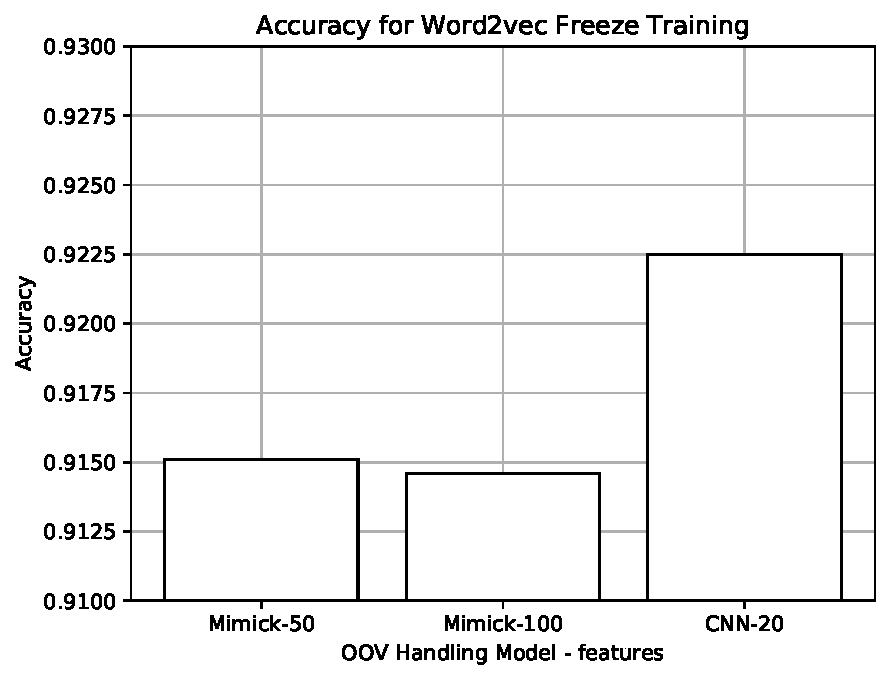
\includegraphics[width=0.8\linewidth]{images/freeze_word2vec.pdf}
        \caption{POS-tagging results frozen embeddings (Word2vec)}
        \label{fig:postag_word2vec_freeze_results}
      \end{figure}
      \begin{figure}[H]
        \centering
        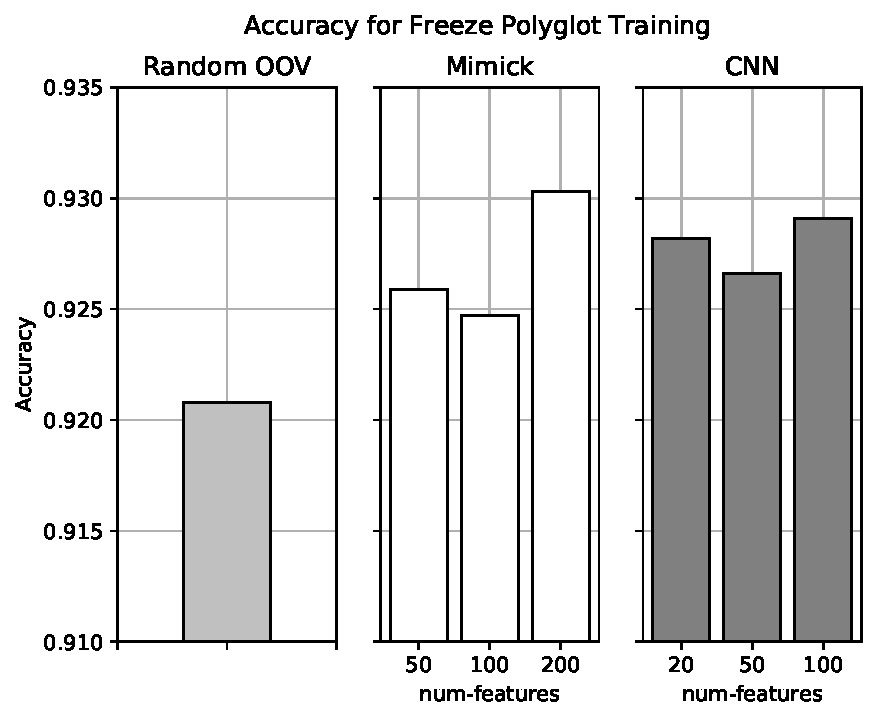
\includegraphics[width=0.8\linewidth]{images/freeze_polyglot.pdf}
        \caption{POS-tagging results frozen embeddings (Polyglot)}
        \label{fig:postag_polyglot_freeze_results}
      \end{figure}
      \begin{figure}[H]
        \centering
        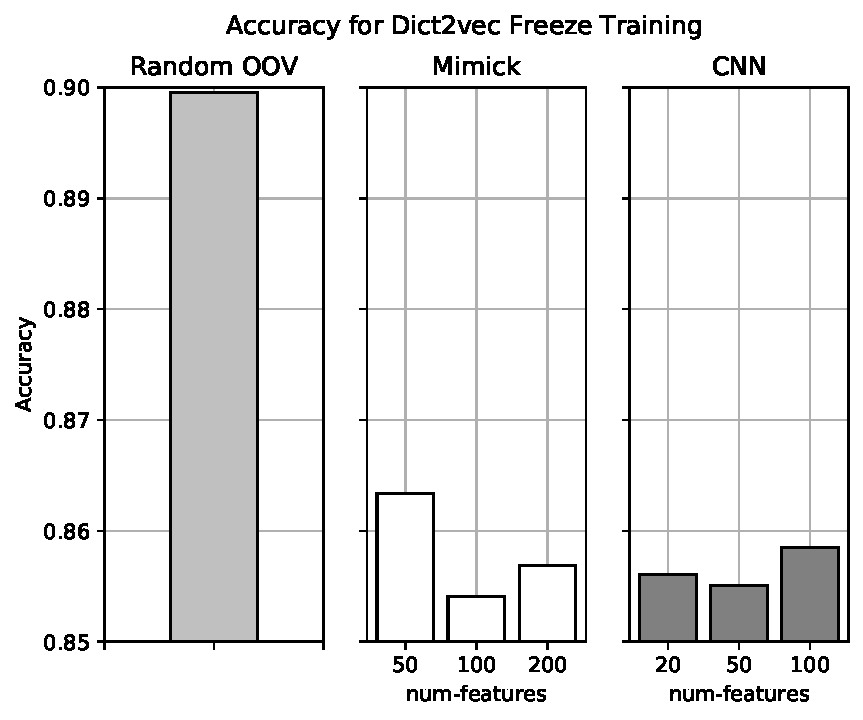
\includegraphics[width=0.8\linewidth]{images/freeze_dict2vec.pdf}
        \caption{POS-tagging results frozen embeddings (Dict2vec)}
        \label{fig:postag_dict2vec_freeze_results}
      \end{figure}
      
      Secondly, the OOV handling model were also trained in
      conjunction with the POS-tagger to improve accuracies of the
      POS-tagger as well as to see whether further improvements in
      accuracies will be achieved by training both the OOV handling
      model and the POS-tagger. Note that the word embedding
      parameters were still untrainable in this setting. The results
      of these experiments were shown in figure
      \ref{fig:postag_word2vec_continuous_results}, figure
      \ref{fig:postag_polyglot_continuous_results}, and figure
      \ref{fig:postag_dict2vec_continuous_results}. The accuracy was
      increased for both OOV handling model as expected surpassing the
      randomly initialized OOV embeddings and the previous setting
      across all pre-trained embeddings. Surprisingly, by allowing the
      OOV handling model to be trained the accuracies of the
      POS-tagger model using CNN as the OOV handling model are
      surpassing the accuracies from POS-tagger that were using
      \textsc{Mimick} as the OOV handling model in all of the
      pre-trained embeddings used in this research.
      \begin{figure}[H]
        \centering
        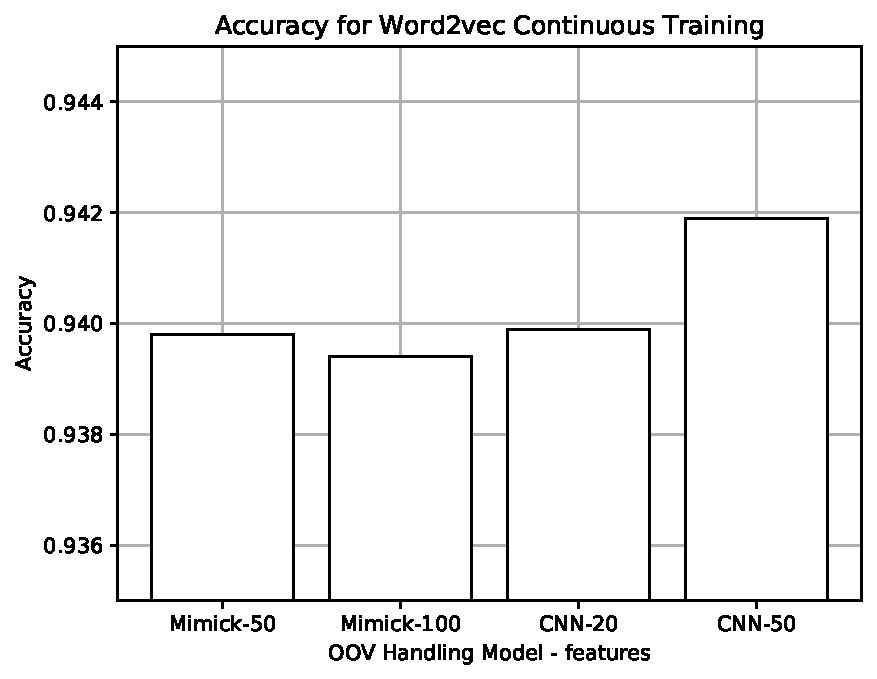
\includegraphics[width=0.8\linewidth]{images/continuous_word2vec.pdf}
        \caption{POS-tagging results continuous embeddings (Word2vec)}
        \label{fig:postag_word2vec_continuous_results}
      \end{figure}
      \begin{figure}[H]
        \centering
        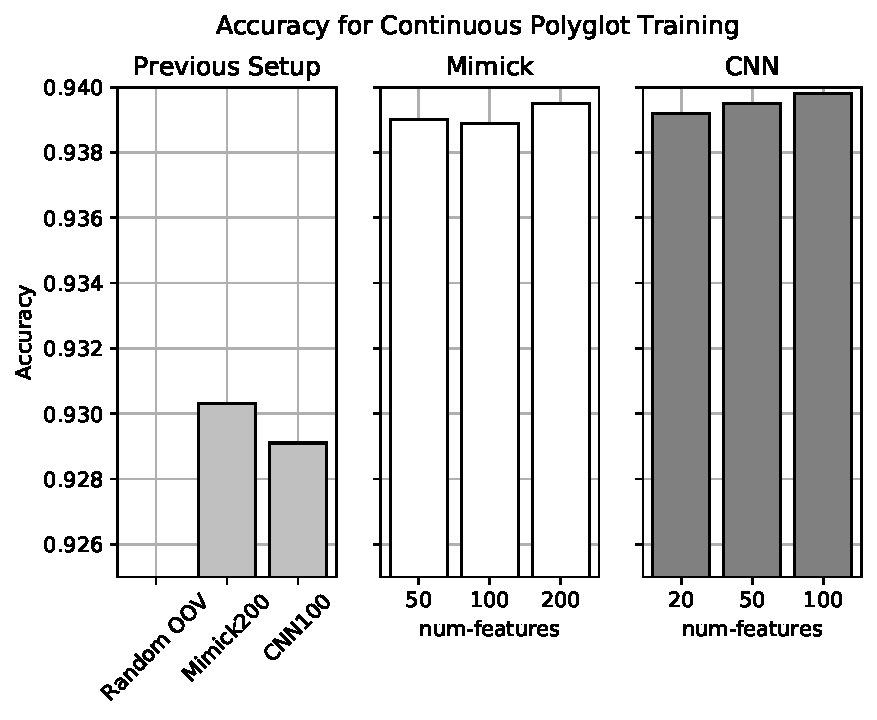
\includegraphics[width=0.8\linewidth]{images/continuous_polyglot.pdf}
        \caption{POS-tagging results continuous embeddings (Polyglot)}
        \label{fig:postag_polyglot_continuous_results}
      \end{figure}
      \begin{figure}[H]
        \centering
        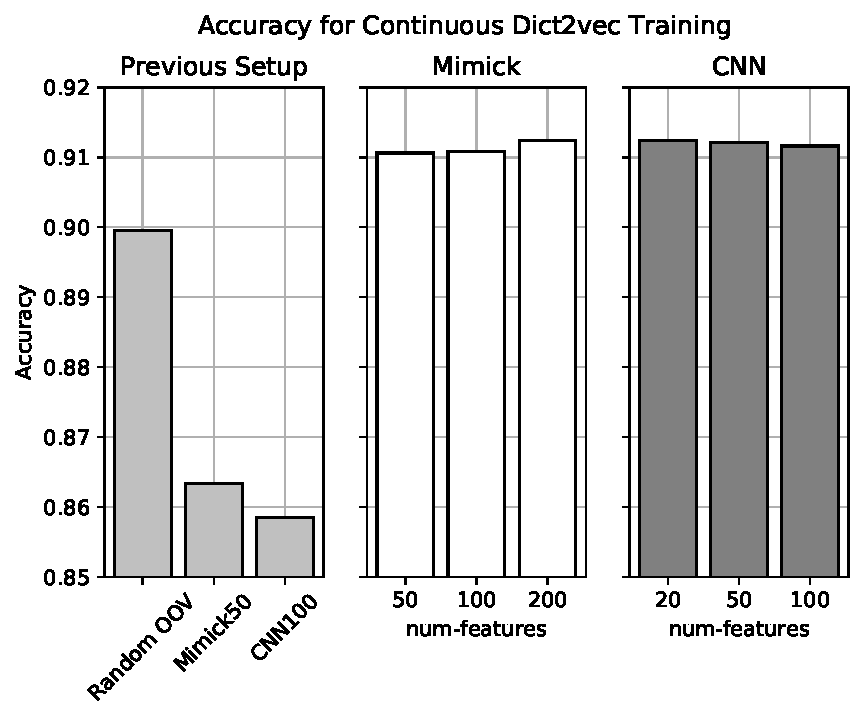
\includegraphics[width=0.8\linewidth]{images/continuous_dict2vec.pdf}
        \caption{POS-tagging results continuous embeddings (Dict2vec)}
        \label{fig:postag_dict2vec_continuous_results}
      \end{figure}

      Thirdly, to simulate how such model will be used in the
      downstream tasks application, both the pre-trained embedding and
      the OOV handling model will be trained and the results will be compared
      to previously stated testing method. The number of features with
      the highest results from each OOV handling model for each word embedding
      were used. The results are shown in figure
      \ref{fig:postag_train_embed_results}. For this setting, CNN
      model were able to outperform \textsc{Mimick} for Polyglot and
      Dict2vec embeddings while it perform worse for Word2vec embedding.
      \begin{figure}[H]
        \centering
        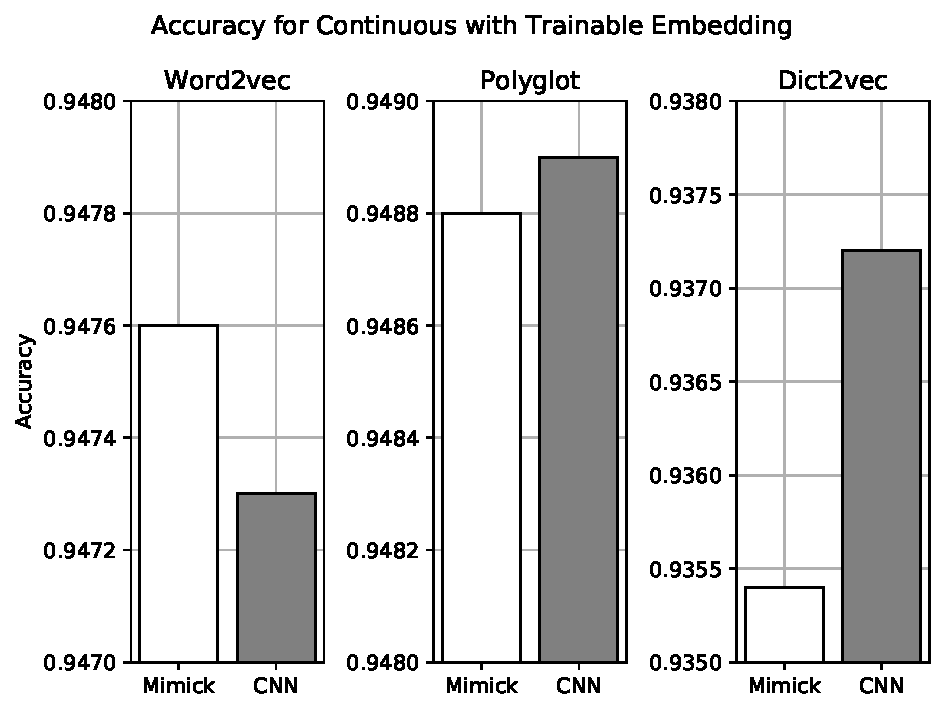
\includegraphics[width=0.8\linewidth]{images/train_embed.pdf}
        \caption{POS-tagging results for OOV handling model and pre-trained embeddings training}
        \label{fig:postag_train_embed_results}
      \end{figure}
      
      Given the results from various settings, in general CNN were
      able to achieve higher accuracies for Brown tag-set dataset.
      Even though \textsc{Mimick} is better at predicting OOV
      embeddings for downstream tasks right \textit{out-of-the-box},
      CNN still outperform \textsc{Mimick} when the OOV handling model
      was also included in the training. This proof that CNN are able
      to learn OOV handling better for  POS-tagging compared to
      bi-LSTM that were used in \textsc{Mimick}.

    \section{Word Similarity}
    For word similarity task, the cosine distance between each given
    pairs from the dataset were calculated. Afterward, Spearman's rank
    correlation coefficient between the predicted embedding cosine
    distance and the score from the dataset were calculated.

    \begin{table}[!ht]
      \begin{threeparttable} 
      \begin{center}
        \caption{Word Similarity Task Results (word2vec)}
        ~\\
        \label{tab:wordsim:word2vec}
        \begin{tabular}{l|c|c|c|c|c}
          \textbf{Dataset} & \textbf{OOV} & \textbf{Invocab} & \textbf{OOV Ratio} & \textbf{Mimick}\tnote{*} & \textbf{CNN}\tnote{*}\\
          \hline
          card & 989 & 317 & 75.73\% & \textbf{52.27} & 27.25\\
          mc30 & 4 & 35 & 10.26\% & 748.11 & \textbf{758.79}\\
          men & 83 & 668 & 11.05\% & \textbf{672.54} & 664.64\\
          mturk287 & 97 & 402 & 19.44\% & 518.15 & \textbf{519.76}\\
          mturk771 & 18 & 1095 & 1.62\% & \textbf{657.93} & 657.04\\
          rg65 & 2 & 46 & 4.17\% & 709.77 & \textbf{732.61}\\
          rwstanford & 1494 & 1457 & 50.63\% & \textbf{233.83} & 217.47\\
          simlex & 20 & 1008 & 1.95\% & 422.77 & \textbf{425.90}\\
          simverb & 90 & 737 & 10.88\% & \textbf{302.37} & 292.91\\
          verb143 & 4 & 113 & 3.42\% & 467.60 & \textbf{478.25}\\
          wordsim & 15 & 422 & 3.43\% & \textbf{658.92} & 648.25\\
          yp130 & 6 & 141 & 4.08\% & \textbf{460.32} & 443.22\\
          \hline
          \multicolumn{4}{r|}{\textbf{average}} & \textbf{492.05} & 488.84\\
        \end{tabular}
        \begin{tablenotes}
          \item[*] multiplied by 1000
        \end{tablenotes}
      \end{center}
      
    \end{threeparttable} 
    \end{table}
    On Table \ref{tab:wordsim:word2vec}, the OOV handling model trained with
    Word2vec \citep{Distributed2013mikolov}. The predicted embedding
    from the OOV handling model with highest accuracy from POS-tagging tasks
    were used for calculating the Spearman's rank correlation $\rho$.
    For easier reading, $\rho$ values were multiplied by 1000. From
    12 word similarity datasets, CNN model has higher Spearman's rank
    correlation coefficient on 5 datasets from 12 datasets with
    averaged Spearman's rank correlation coefficient of $488.84$ compared to
    \textsc{Mimick} that achieved $492.05$. The higher $\rho$ values
    for each model and each dataset were marked with bold type setting
    in the table.

    \begin{table}[!ht]
      \begin{threeparttable} 
      \begin{center}
        \caption{Word Similarity Task Results (polyglot)}
        ~\\
        \label{tab:wordsim:polyglot}
        \begin{tabular}{l|c|c|c|c|c}
          \textbf{Dataset} & \textbf{OOV} & \textbf{Invocab} & \textbf{OOV Ratio} & \textbf{Mimick}\tnote{*} & \textbf{CNN}\tnote{*}\\
          \hline
          card & 864 & 442 & 66.16\% & \textbf{128.93} & 114.11\\
          mc30 & 1 & 38 & 2.56\% & 605.25 & 605.25\\
          men & 14 & 737 & 1.86\% & 490.57 & \textbf{492.17}\\
          mturk287 & 76 & 423 & 15.23\% & 443.31 & \textbf{458.81}\\
          mturk771 & 3 & 1110 & 0.27\% & \textbf{432.48} & 432.20\\
          rg65 & 1 & 47 & 2.08\% & 531.59 & \textbf{524.77}\\
          rwstanford & 999 & 1952 & 33.85\% & 272.33 & \textbf{290.78}\\
          simlex & 4 & 1024 & 0.39\% & 232.20 & \textbf{234.16}\\
          simverb & 53 & 774 & 6.41\% & \textbf{137.01} & 134.42\\
          verb143 & 0 & 117 & 0.00\% & 335.81 & 335.81\\
          wordsim & 0 & 437 & 0.00\% & 412.83 & 412.83\\
          yp130 & 5 & 142 & 3.40\% & \textbf{44.76} & 44.62\\
          \hline
          \multicolumn{4}{r|}{average} & 338.92 & \textbf{339.99}\\
        \end{tabular}
        \begin{tablenotes}
          \item[*] multiplied by 1000
        \end{tablenotes}
      \end{center}
    \end{threeparttable} 
    \end{table}

    The same procedure was used for both models trained with polyglot
    \citep{polyglot2013alrfou}. From 12 word similarity datasets,
    \textsc{Mimick} has 4 datasets that has higher Spearman's rank
    correlation coefficient than CNN model and 5 datasets that is
    lower compared to CNN model while the other 2 has similar $\rho$
    value because of no OOV entries. In contrast with the model
    trained with word2vec, the model trained with polyglot
    \citep{polyglot2013alrfou} only achieved Spearman's rank
    correlation coefficient as high as $338.92$ and $339.99$ for
    \textsc{Mimick} and CNN respectively, giving results that CNN has
    higher $\rho$ value compared to \textsc{Mimick} as shown on Table
    \ref{tab:wordsim:polyglot}.

    \begin{table}[!ht]
      \begin{threeparttable} 
      \begin{center}
        \caption{Word Similarity Task Results (Dict2vec)}
        ~\\
        \label{tab:wordsim:dict2vec}
        \begin{tabular}{l|c|c|c|c|c|c}
          \textbf{Dataset} & \textbf{OOV} & \textbf{Invocab} &
          \textbf{OOV Ratio} & \textbf{Random}\tnote{*} &
          \textbf{Mimick}\tnote{*} & \textbf{CNN}\tnote{*}\\
          \hline
          card & 828 & 478 & 63.40\% & 48.07 & 80.89 & \textbf{95.32}\\
          mc30 & 0 & 39 & 0.00\% & 847.57 & 847.57 & 847.57\\
          men & 1 & 750 & 0.13\% & 713.16 & 723.63 & \textbf{723.89}\\
          mturk287 & 2 & 497 & 0.40\% & 652.27 & \textbf{655.32} & 653.13\\
          mturk771 & 0 & 1113 & 0.00\% & 683.91 & 683.91 & 683.91\\
          rg65 & 0 & 48 & 0.00\% & 832.86 & 832.86 & 832.86\\
          rwstanford & 619 & 2332 & 20.98\% & 214.60 & \textbf{403.79} & 400.27\\
          simlex & 3 & 1025 & 0.29\% & 454.80 & \textbf{460.66} & 459.87\\
          simverb & 24 & 803 & 2.90\% & 375.15 & 390.09 & \textbf{393.39}\\
          verb143 & 0 & 117 & 0.00\% & 187.82 & 187.82 & 187.82\\
          wordsim & 18 & 419 & 4.12\% & 642.71 & 718.72 & \textbf{723.72}\\
          yp130 & 2 & 145 & 1.36\% & 577.76 & 621.38 & \textbf{621.75}\\
          \hline
          \multicolumn{4}{r|}{average} & 519.22 & 550.55 & \textbf{551.96}\\
        \end{tabular}
        \begin{tablenotes}
          \item[*] multiplied by 1000
        \end{tablenotes}
      \end{center}
    \end{threeparttable} 
    \end{table}

    For baseline embedding Dict2vec \citep{dict2vect2017tissier}. The
    original embedding added with randomly generated embedding for OOV
    handling were tried five times and the one with highest results
    for each dataset was selected. The results then compared with CNN
    and \textsc{Mimick} models. Dict2vec only able to achieve
    Spearman's rank correlation coefficient of $519.22$. In contrast to
    \textsc{Mimick} model and CNN model were able to achieve $550.55$
    and $551.96$ on average respectively as shown on Table
    \ref{tab:wordsim:dict2vec}. This shows that both OOV handling
    models can handle OOV better than initializing embedding randomly
    for OOV. On top of that, for Dict2vec word embedding, CNN performs
    better than \textsc{Mimick}.

    In summary, for word similarity tasks over 12 datasets and 3
    pre-trained word embeddings CNN performs better on Polyglot and
    Dict2vec while \textsc{Mimick} performs better on word2vec in word
    similarities tasks. This further proved that CNN are better for
    handling OOV than \textsc{Mimick}.